\documentclass[a4paper]{article}

\usepackage{polski}
\usepackage[utf8]{inputenc}
\usepackage{amsmath}
\usepackage{graphicx}
\usepackage[colorinlistoftodos]{todonotes}

\usepackage{float}

\usepackage{listings}

\title{Opis zadania 8.1}

\author{Przemysław Sagało}

\date{\today}

\begin{document}
\maketitle
\section{Specyfikacja problemu}   
Równanie postaci:
\begin{equation}
a \cdot x + b \cdot y+c = 0 
\end{equation}
nazywamy \textbf{równaniem ogólnym prostej}. 
Równanie to zależy od wartości trzech współczynników $a$, $b$ i $c$.
W zależności od wartości tych współczynników równanie to może wystąpić w ośmiu postaciach. \\
W przypadku gdy wszystkie współczynniki są równe 0, równanie to jest zawsze spełnione.\\
Jeżeli $a=b=0$ oraz $c\neq0$ to równanie jest sprzeczne.\\
Gdy $b\neq0$ a pozostałe współczynniki są równe 0, to $x$ jest dowolne a $y=0$.\\
W przypadku gdy tylko współczynnik $a=0$, to $x$ jest dowolne a $y = \frac{-c}{b}$.\\
Gdy tylko $a\neq0$, to $x=0$ i $y$ jest dowolne.\\
Jeżeli tylko $b=0$, to $x = -\frac{c}{a}$ i $y$ jest dowolny.\\
Dla $c=0$, $y=\frac{-a}{x} \cdot x$ z kolei jeżeli wszystkie współczynniki są różne od zera to $y=\frac{-a}{b} \cdot x - \frac{c}{b}$.   

W ujęci geometrycznym jeżeli współczynnik $a = 0$, to prosta jest równoległa do osi $Ox$, jeżeli współczynnik $b=0$, to prosta jest równoległa do osi $Oy$ z kolei gdy $c=0$, to prosta przechodzi przez środek układu współrzędnych.
Jeżeli współczynniki $a$ i $b$ są równocześnie równe zeru, wtedy równanie to nie opisuje prostej, lecz w przypadku gdy $c=0$ równanie to opisuje całą płaszczyznę, a dla $c \neq 0$ jest sprzeczne.


\section{List kroków}
\begin{enumerate}
\item if a == 0 and b == 0 and c == 0:
    równanie jest zawsze spełnione
\item elif a == 0 and b == 0 and c != 0:
    rownanie jest sprzeczne
\item elif a == 0 and b != 0 and c == 0:
    x - dowolne, y=0
\item elif a == 0 and b != 0 and c != 0:
    x - dowolne, y=$-c/b$
\item elif a != 0 and b == 0 and c == 0:
    x=0, y - dowolne
\item elif a != 0 and b == 0 and c != 0:
    x=-c/float(a), y - dowolne
\item elif a != 0 and b != 0 and c == 0:
    y=-a/b x
\item elif a != 0 and b != 0 and c != 0:
    y=$-a/b x  -c/b$
\end{enumerate}

\section{Schemat blokowy}
\begin{figure}[H]
	\begin{center}
		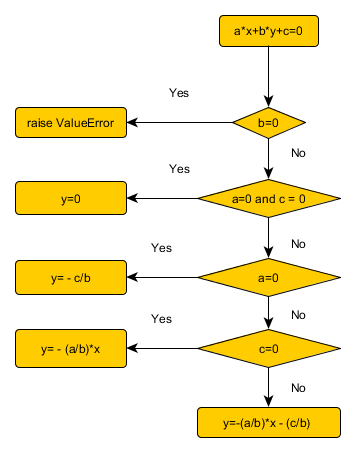
\includegraphics[width=11cm]{block_diagram.png}
		\caption{Schemat blokowy powyższego zagadnienia.}
	\end{center}	
\end{figure}

\section{Schemat w postaci drzewa}
\begin{figure}[H]
	\begin{center}
		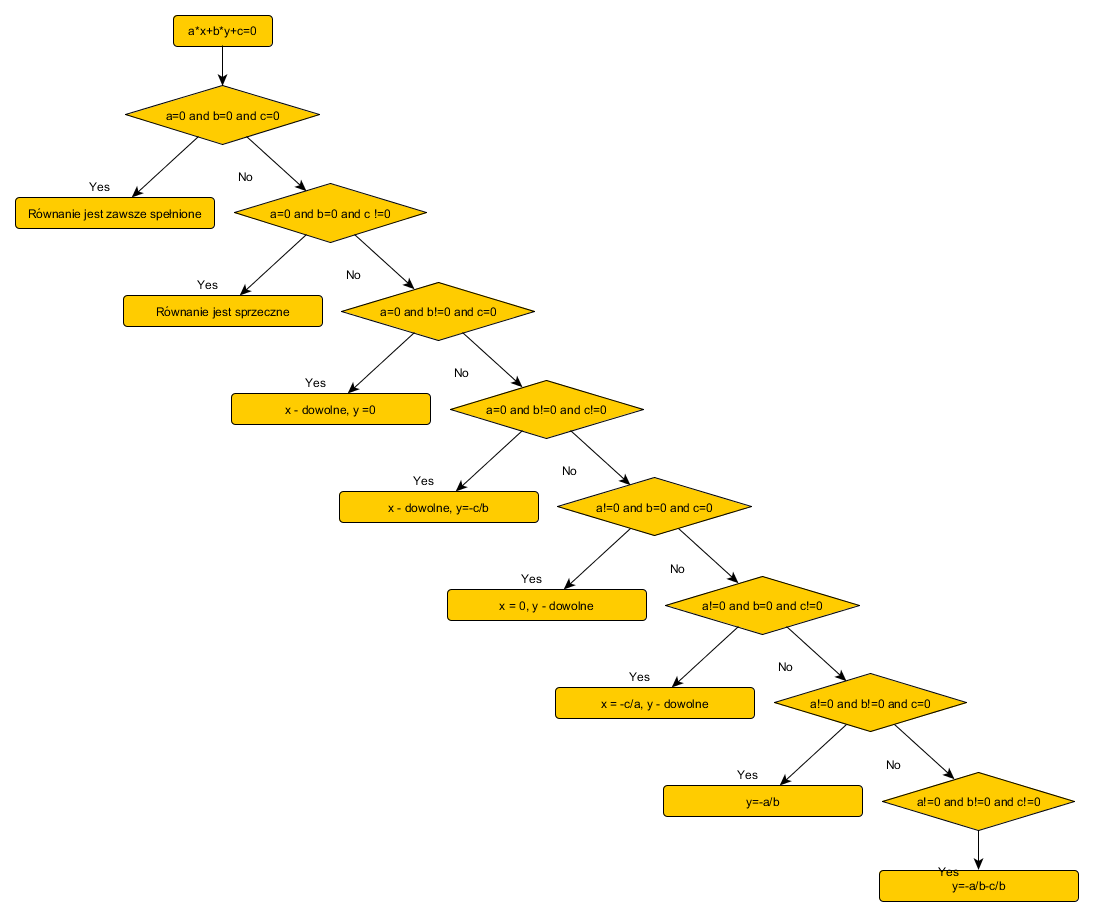
\includegraphics[width=15cm]{tree_diagram.png}
		\caption{Schemat w postaci drzewa dla powyższego zagadnienia.}
	\end{center}	
\end{figure}
\newpage

\section{Algorytm}
\begin{lstlisting}[language=Python]
def solve1(a, b, c):
    """Rozwiazywanie rownania liniowego a x + b y + c = 0."""
    if a == 0 and b == 0 and c == 0:
        to_return = 'rownanie jest zawsze spelnione'
    elif a == 0 and b == 0 and c != 0:
        to_return = 'rownanie jest sprzeczne'
    elif a == 0 and b != 0 and c == 0:
        to_return = 'x - dowolne, y=0'
    elif a == 0 and b != 0 and c != 0:
        to_return = 'x - dowolne, y={}'.format(-c/float(b))
    elif a != 0 and b == 0 and c == 0:
        to_return = 'x=0, y - dowolne'
    elif a != 0 and b == 0 and c != 0:
        to_return = 'x={}, y - dowolne'.format(-c/float(a))
    elif a != 0 and b != 0 and c == 0:
        to_return = 'y={} x'.format(-a/float(b))
    elif a != 0 and b != 0 and c != 0:
        to_return = 'y={0} x {1}'.format(-a/float(b), -c/float(b))

    return to_return

\end{lstlisting}

\end{document}